\documentclass[a4paper,12pt]{article}

\usepackage{subcaption}
\usepackage{pgfplots}
\usepackage{tikz}

\begin{document}
  
\begin{figure}
  \begin{subfigure}[t]{0.48\textwidth}
    \centering
    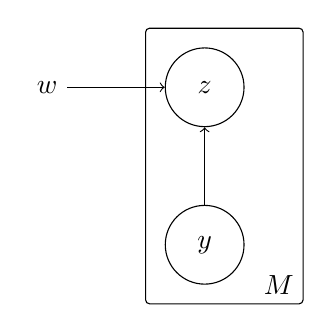
\begin{tikzpicture}

      \node[rectangle,rounded corners=0.05cm,draw=black,minimum width=2cm,minimum height=3.5cm] (M) at (0.25, -1){};
      \node[above left] at (M.south east){$M$};
      \node[circle,draw=black,minimum size=1cm] (z) at (0,0){$z$};
      \node[circle,draw=black,minimum size=1cm] (y) at (0,-2){$y$};
      \node[] (w) at (-2,0){$w$};
      
      \draw[->] (w) -- (z);
      \draw[->] (y) -- (z);
      
    \end{tikzpicture}
    \caption{}
  \end{subfigure}\hfill
  \begin{subfigure}[t]{0.48\textwidth}
    \centering
    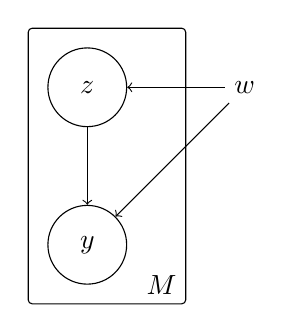
\begin{tikzpicture}

      \node[rectangle,rounded corners=0.05cm,draw=black,minimum width=2cm,minimum height=3.5cm] (M) at (0.25, -1){};
      \node[above left] at (M.south east){$M$};
      \node[circle,draw=black,minimum size=1cm] (z) at (0,0){$z$};
      \node[circle,draw=black,minimum size=1cm] (y) at (0,-2){$y$};
      \node[] (w) at (2,0){$w$};
      
      \draw[->] (w) -- (z);
      \draw[->] (w) -- (y);
      \draw[->] (z) -- (y);

    \end{tikzpicture}
    \caption{}
  \end{subfigure}
\end{figure}

\begin{figure}
  \centering
  \begin{subfigure}[t]{0.48\textwidth}
    \centering
    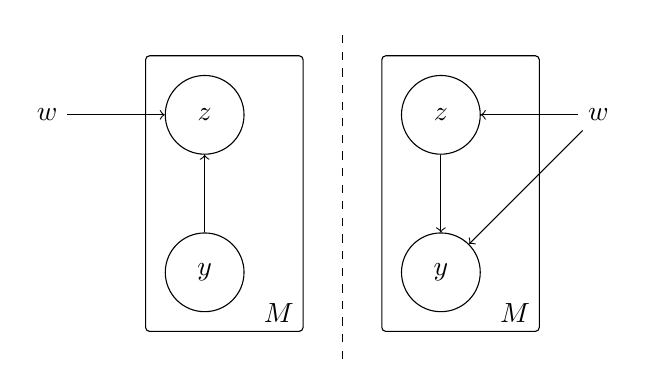
\begin{tikzpicture}

      \node[rectangle,rounded corners=0.05cm,draw=black,minimum width=2cm,minimum height=3.5cm] (M) at (0.25, -1){};
      \node[above left] at (M.south east){$M$};
      \node[circle,draw=black,minimum size=1cm] (z) at (0,0){$z$};
      \node[circle,draw=black,minimum size=1cm] (y) at (0,-2){$y$};
      \node[] (w) at (-2,0){$w$};
      
      \draw[->] (w) -- (z);
      \draw[->] (y) -- (z);
      
      \draw[-,dashed] (1.75,-3.1) -- (1.75,1.1);
      
      \node[rectangle,rounded corners=0.05cm,draw=black,minimum width=2cm,minimum height=3.5cm] (M) at (3.25, -1){};
      \node[above left] at (M.south east){$M$};
      \node[circle,draw=black,minimum size=1cm] (z) at (3,0){$z$};
      \node[circle,draw=black,minimum size=1cm] (y) at (3,-2){$y$};
      \node[] (w) at (5,0){$w$};
      
      \draw[->] (w) -- (z);
      \draw[->] (w) -- (y);
      \draw[->] (z) -- (y);
      
    \end{tikzpicture}
    \caption{}
  \end{subfigure}\hfill
  \begin{subfigure}[t]{0.48\textwidth}
    \centering
    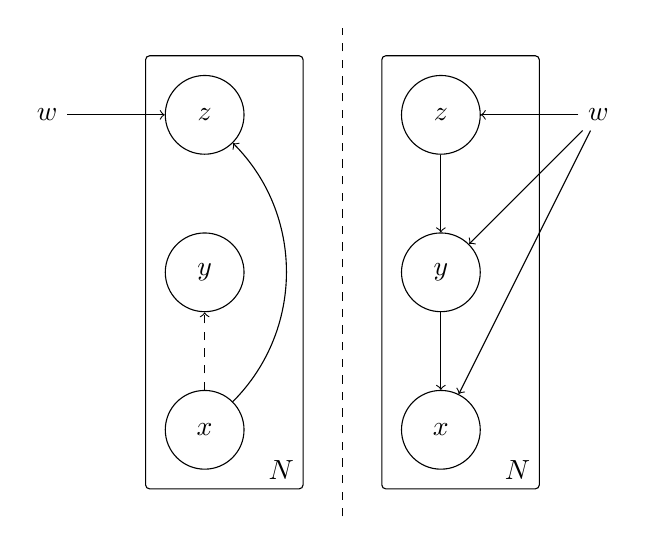
\begin{tikzpicture}

      \node[rectangle,rounded corners=0.05cm,draw=black,minimum width=2cm,minimum height=5.5cm] (M) at (0.25, -2){};
      \node[above left] at (M.south east){$N$};
      \node[circle,draw=black,minimum size=1cm] (z) at (0,0){$z$};
      \node[circle,draw=black,minimum size=1cm] (y) at (0,-2){$y$};
      \node[circle,draw=black,minimum size=1cm] (x) at (0,-4){$x$};
      \node[] (w) at (-2,0){$w$};
      
      \draw[->] (w) -- (z);
      %\draw[->] (y) -- (z);
      \draw[->,dashed] (x) -- (y);
      \draw[->] (x) to [out=45,in=315](z);
      
      \draw[-,dashed] (1.75,-5.1) -- (1.75,1.1);
      
      \node[rectangle,rounded corners=0.05cm,draw=black,minimum width=2cm,minimum height=5.5cm] (M) at (3.25, -2){};
      \node[above left] at (M.south east){$N$};
      \node[circle,draw=black,minimum size=1cm] (z) at (3,0){$z$};
      \node[circle,draw=black,minimum size=1cm] (y) at (3,-2){$y$};
      \node[circle,draw=black,minimum size=1cm] (x) at (3,-4){$x$};
      \node[] (w) at (5,0){$w$};
      
      \draw[->] (w) -- (z);
      \draw[->] (w) -- (y);
      \draw[->] (w) -- (x);
      \draw[->] (z) -- (y);
      \draw[->] (y) -- (x);

    \end{tikzpicture}
    \caption{}
  \end{subfigure}
\end{figure}

\end{document}